\section{Simplified ByteNet}

\subsection{Performance Profiling}


\begin{figure}[h]
    \centering
    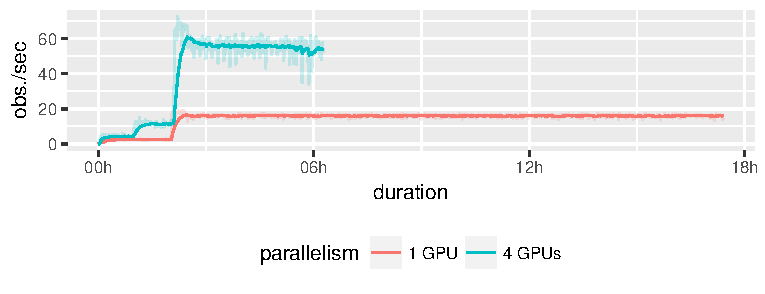
\includegraphics[scale=1]{bytenet-small/timing-gpus.pdf}
    \caption{Comparing observations per second, depending on the number of GPUs used.}
    \label{fig:result:bytenet:timing-gpus}
\end{figure}

\begin{figure}[h]
    \centering
    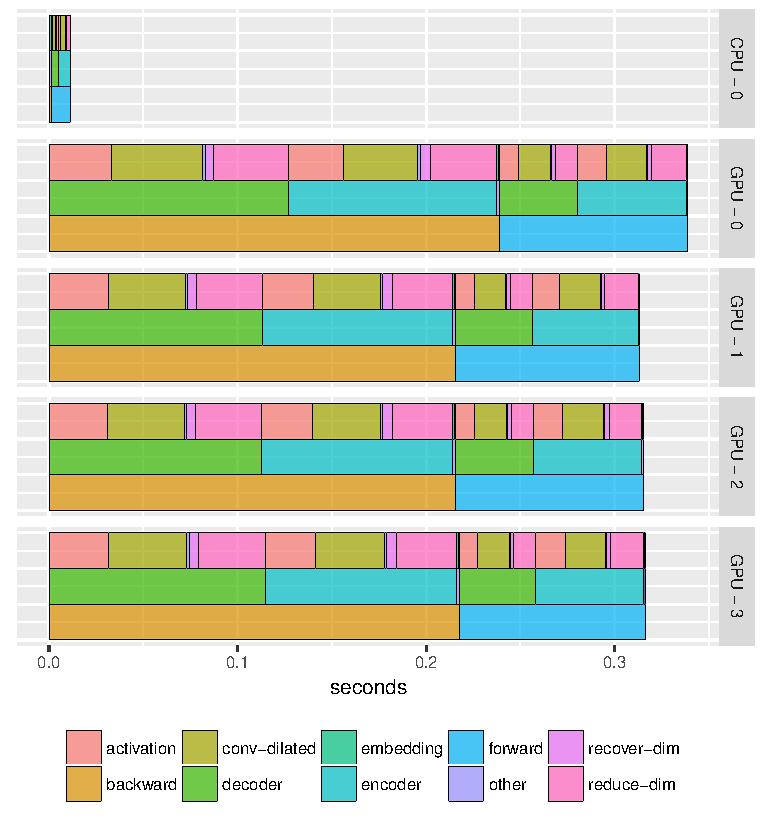
\includegraphics[scale=1]{bytenet-small/profile-grouped-gpu4.pdf}
    \caption{Shows time spend executing operations in each part of the ByteNet model, this excludes the waiting time. Each part exists in a hierarchy, which is visualized as levels. The bottom level is the least detailed level, it just splits the model in the backward and forward pass. The next level, splits the model in the encoder and decoder. The last level at the top, primarily splits the Simplified ByteNet Residual Blocks.}
    \label{fig:result:bytenet:profile-raw}
\end{figure}

\subsection{WMT Translation Task}

